\begin{frame}[c]\frametitle{Intergroup Bias}


    \ex.\label{ex:intro-1} \a. \alert{\textbf{Admire}} Chairman @reprichmond’s moral voice on issues of racism and restorative justice. He is \alert{\textbf{a real leader}} for our nation and Congress.
    \b. Parents and families live in constant fear for their children with food allergies. A worthy \alert{\textbf{bipartisan}} cause - thank you @drphilroe for your \alert{\textbf{leadership}} on this issue.

    \pause\vfill

    These utterances differ along two \textbf{interpersonal} dimensions:
    
    \begin{itemize}
        \item the relationship between speaker and target --- (a) is \textbf{in-group}, (b) is \textbf{out-group}.
        \item emotion expressed by speaker towards target.
    \end{itemize}

\end{frame}


% \begin{frame}[plain, standout]\frametitle{}
%     Analyze and model 2 dimensions of intergroup bias --- \textbf{intergroup relationship} and \textbf{interpersonal emotion}.\pause
% 
%     \vspace{\baselineskip}
%     
%     How does intergroup relationship (in-group vs. out-group) \textbf{interact} with interpersonal emotion?
% 
% \end{frame}

% \begin{frame}[c]\frametitle{Data}
%     \vfill
%     \begin{itemize}
%         \itemsep=2em
%         \item Tweets by members of US Congress which mention one other member. \pause
%         \item Tweets are either directed in-group or out-group.
%     \end{itemize}
%    \pause
%    \vfill
%    \centering
%    {\Large\textbf{3033}} (identity masked) tweets annotated for fine-grained emotion using Plutchik wheel, with \emph{found supervision} for intergroup relationship labels.
% 
%    \blfootnote{\cite{plutchik2001nature}}
%       
% \end{frame}

\begin{frame}[c]\frametitle{Emotion distribution}

   \pause
    
    \begin{figure}
        \begin{tikzpicture}
   \begin{axis}[
       xbar stacked,
       cycle list name=mbarplot cycle,
       width  = \columnwidth,
       height = 0.8\textheight,
       major x tick style = transparent,
       bar width=40pt,
       axis y line*=left,
       x axis line style={draw opacity=0},
       xmajorgrids=true,
       y tick style={draw=none},
       x tick style={draw=none},
       tick label style={/pgf/number format/assume math mode=true, font=\normalsize},
       xlabel={},
       symbolic y coords={Out-group, In-group, All},
       ytick = data,
       yticklabel style={rotate=90},
       extra y tick style={grid=none},
       xmin=0,
       xmax=100,
       xtick={0,100},
       scaled y ticks = false,
       enlarge y limits=0.1,
       legend cell align=left,
       legend columns=-1,
       legend style={
            fill=none,
               draw=none,
               at={(0.5,1.2)},
               anchor=north,
               text=black,
               font=\normalsize,
               /tikz/every even column/.append style={column sep=0.5cm}
        },
        nodes near coords,
        nodes near coords style={font=\small, text=white,/pgf/number format/assume math mode}
   ]
       \addplot+[xbar, draw=none]
           coordinates {(31.4,All) (35.8,In-group) (27.1,Out-group)};

       \addplot+[xbar, draw=none]
           coordinates {(22.7,All) (31.2,In-group) (14.1,Out-group)};

       \addplot+[xbar, draw=none]
           coordinates {(3.8,All) (3.9,In-group) (3.7,Out-group)};

       \addplot+[xbar, draw=none]
           coordinates {(8.9,All) (0.0,In-group) (17.7,Out-group)};

       \addplot+[xbar, draw=none]
           coordinates {(9.3,All) (0.0,In-group) (18.4,Out-group)};

        \addplot+[xbar, draw=none]
           coordinates {(23.8,All) (28.9,In-group) (18.9,Out-group)};

       \legend{Joy, Admiration, Sadness, Disgust, Anger, Interest}
   \end{axis}
\end{tikzpicture}

        \label{fig:emot-dist}
    \end{figure}

\end{frame}


\begin{frame}[c]\frametitle{Tweet Embeddings \& Gold Emotions}
    
    \pause
    
    \begin{figure}
        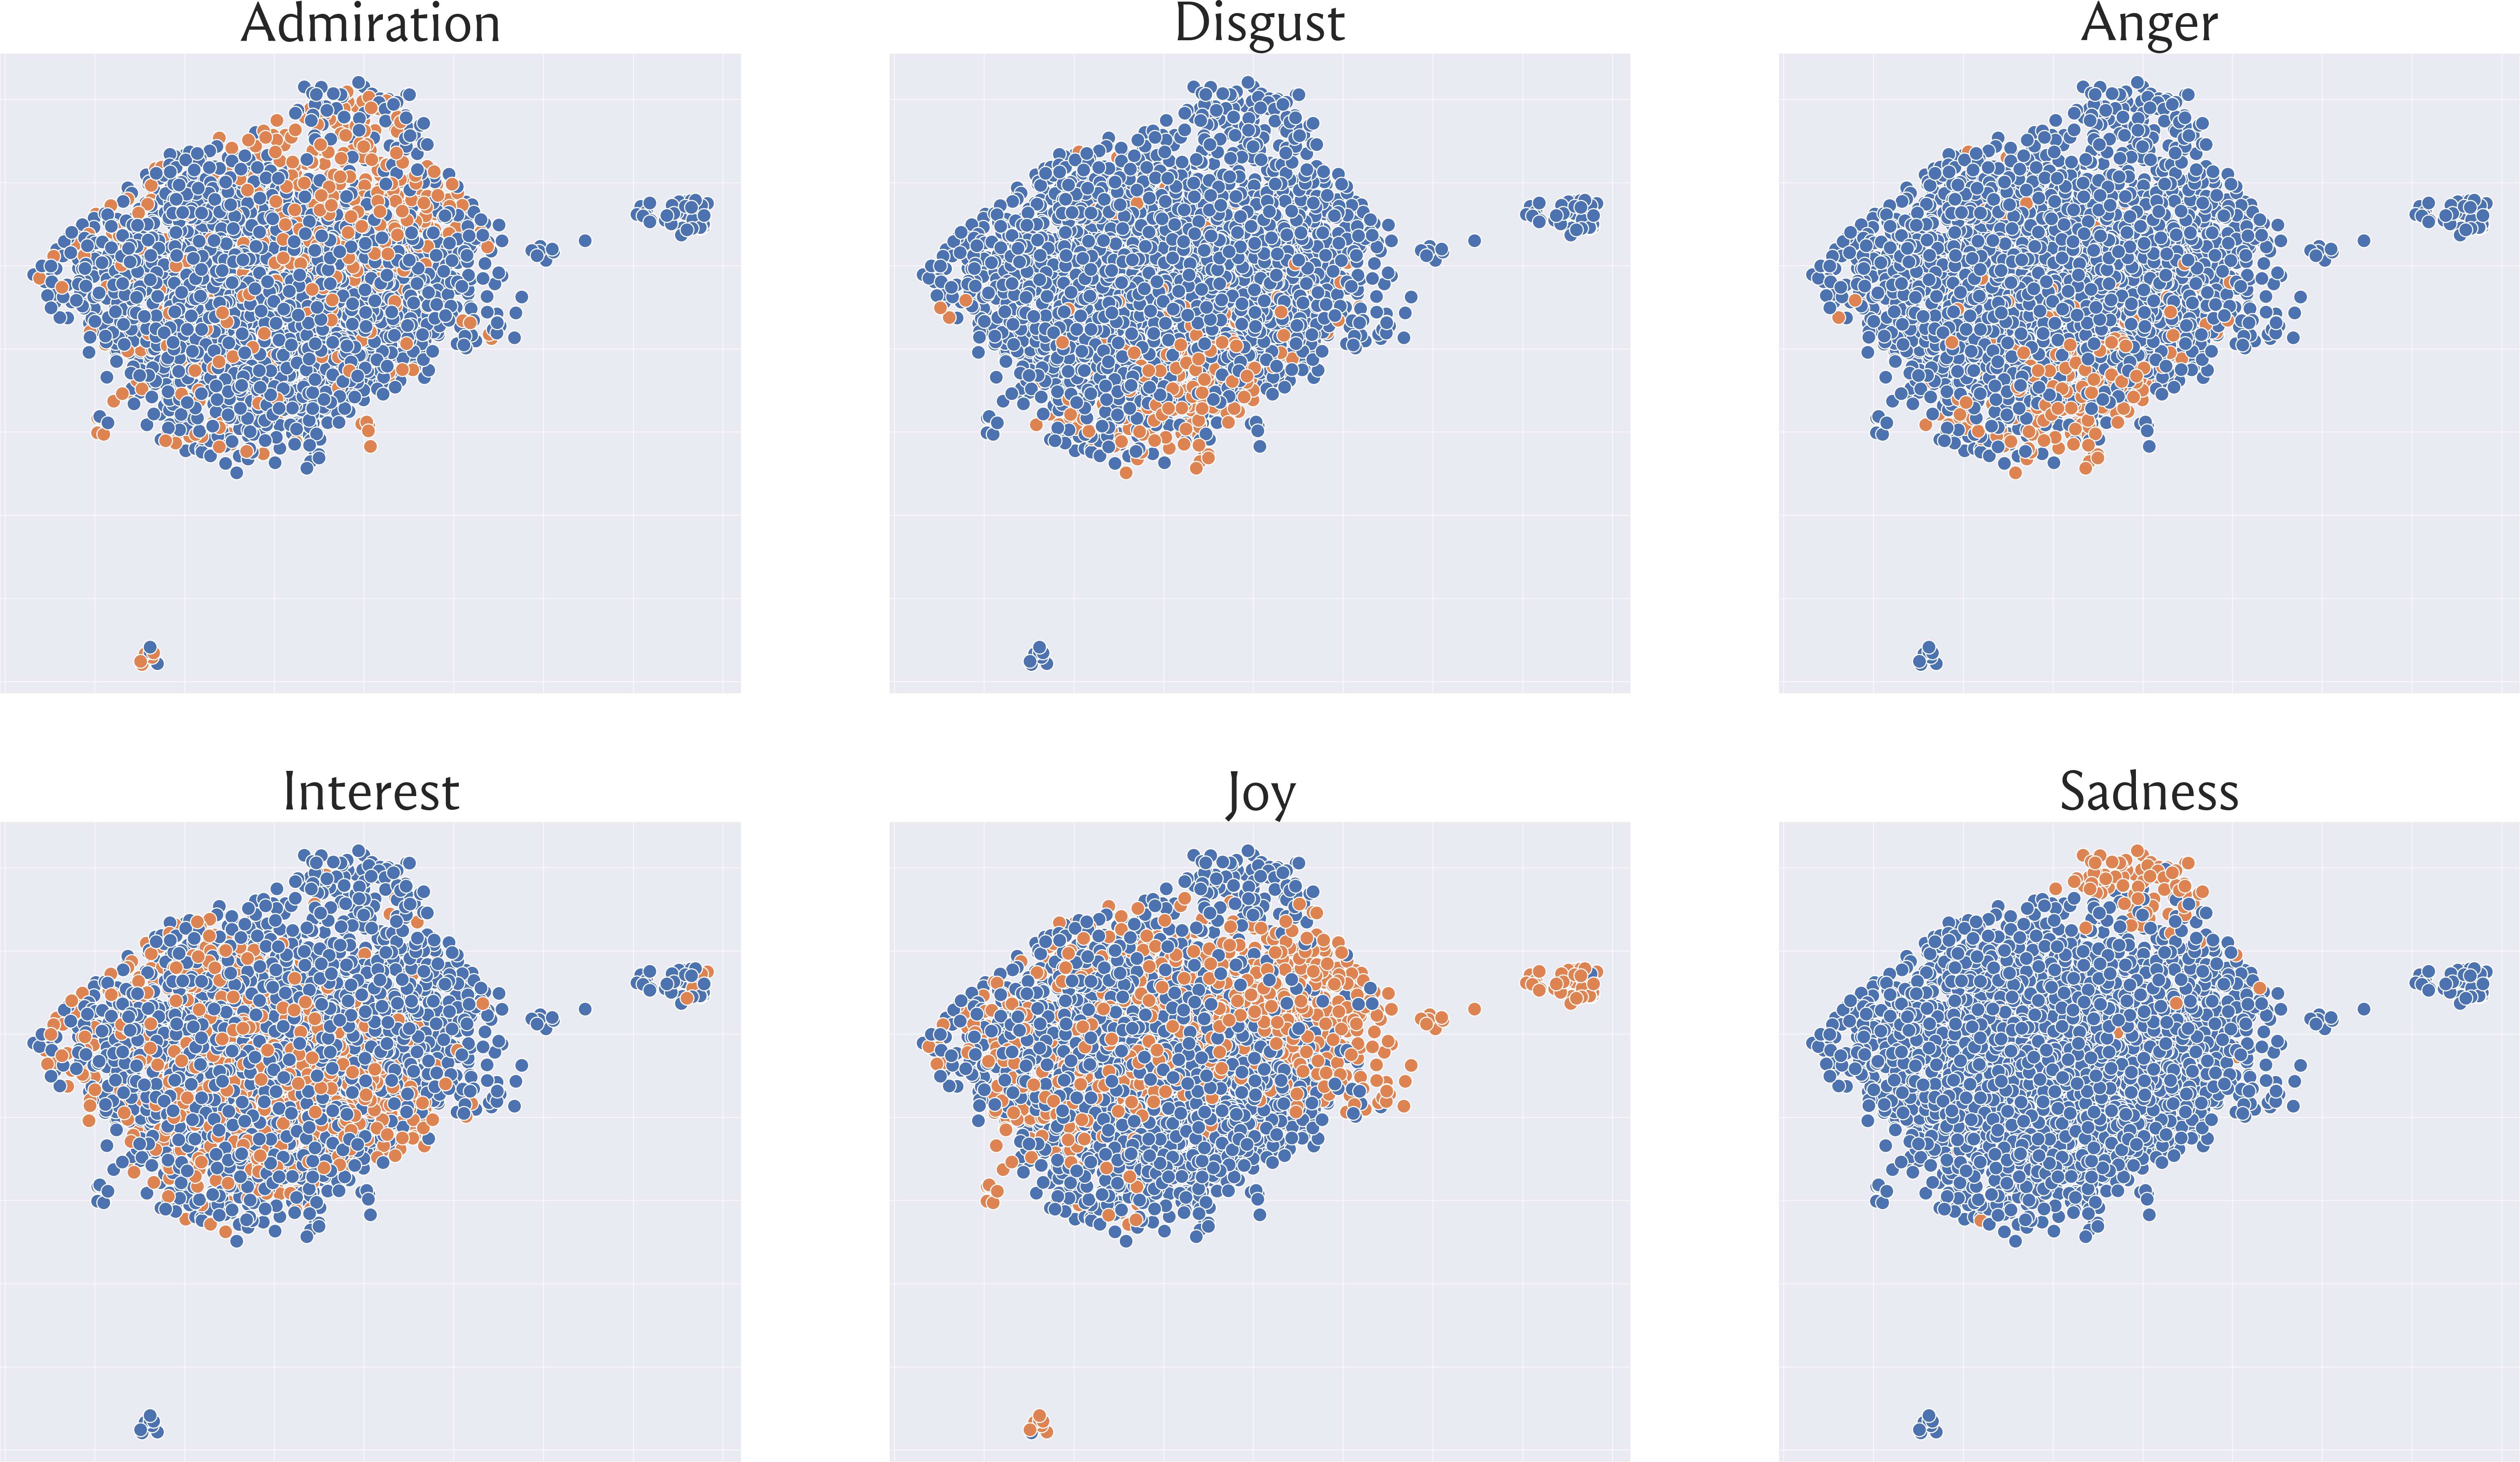
\includegraphics[width=0.93\columnwidth]{bt_emots.png}
        \caption{\small Tweet embeddings from a language model projected downward to 2 dimensions. Each point is a tweet and \textcolor{orange}{orange} indicates the emotion is present. Observe the separability of clusters of emotions.}
        \label{fig:emots_bt}
    \end{figure}
    \nocite{sainburg2021parametric}
    
\end{frame}

\begin{frame}[c]\frametitle{Results}
    \begin{figure}
    \begin{tikzpicture}
        \begin{axis}[
            ybar=0pt,
            cycle list name=mbarplot cycle,
            width  = \columnwidth,
            height = 0.8\textheight,
            major x tick style = transparent,
            xtick = data,
            extra x tick style={grid=none},
            y tick style={draw=none},
            tick label style={/pgf/number format/assume math mode=true},
            scaled y ticks = false,
            bar width=30pt,
            axis x line*=bottom,
            y axis line style={draw opacity=0},
            ymajorgrids=true,
            symbolic x coords={Baseline, BERTweet, Multitask},
            enlarge x limits=0.2,
            grid style={black!30},
            ymin=0,
            ymax=100,
            legend cell align=left,
            legend columns=-1,
            legend style={
                    at={(0.5,1.15)},
                    anchor=north,
                    text=fgcolor,
                    font=\small,
                    draw=none,
                    fill=none,
                    /tikz/every even column/.append style={column sep=0.5cm}
            },
            nodes near coords,
            nodes near coords style={font=\small, text=fgcolor,/pgf/number format/assume math mode}
        ]
        \addplot+[fill opacity=1, visible on=<2->,draw=none, error bars/.cd, y dir=both, y explicit, error bar style={line width=1pt}, error mark options={TolDarkBlue, rotate=90, mark size=4pt, line width=1pt}]
                coordinates {(Baseline, 62.5) (BERTweet, 74.1)+-(0,3.3) (Multitask, 77.3)+-(0,0.8) };
        \addplot+[fill opacity=1, visible on=<3->,draw=none, error bars/.cd, y dir=both, y explicit, error bar style={line width=1pt}, error mark options={TolLightBrown, rotate=90, mark size=4pt, line width=1pt}]
                coordinates {(Baseline, 24.8) (BERTweet, 68.5)+-(0,1.9) (Multitask, 69.7)+-(0,0.6) };
        \legend{Intergroup Relationship, Interpersonal Emotion}
        \end{axis}
    \end{tikzpicture}
    \caption{\onslide<3->{Recall score. Multitasking improves on vanilla model (slightly).}}
\end{figure}

\end{frame}


\begin{frame}[c]\frametitle{Takeaways}

    \begin{itemize}
      \itemsep=\baselineskip
       \item Interpersonal emotion and intergroup relationship, two dimensions of intergroup bias, co-vary systematically.\pause
       \item Multitask modeling provides further evidence that the two are intertwined.\pause
      \item What is the actual \textbf{linguistic variation}? How does it interact with \textbf{situational context}? 
    \end{itemize}

\end{frame}
